\documentclass[a4paper,kulak]{kulakarticle}

\usepackage[dutch]{babel}
\usepackage{hyperref}
\usepackage{graphicx}
\usepackage{amsmath, amssymb, amsthm}
\usepackage{siunitx}
\usepackage[toc,page]{appendix}
\renewcommand\appendixname{Bijlage}
\renewcommand\appendixpagename{Bijlagen}
\usepackage{pdfpages}


\title{Tussentijds verslag}
\author{Groep 1}
\date{\today}

\begin{document}

\maketitle
\tableofcontents

\newpage

\section{Inleiding}

\subsection{Probleemstelling}
Meer en meer zien we een groei van het verstedelijkt gebied. De verstedelijking breidt zich uit en de groei wordt versterkt. Met deze groei nemen ook de problemen toe, criminaliteit, lawaai, milieuvervuiling en zoveel meer. Als we terugkijken in de tijd, zien we een meermaals voorkomende situatie. Steden zitten in een bloeiperiode, bereiken een verzadingspunt en vallen dan ineen. Zo was er ook de val van Rome, nadat deze een hoogtepunt had bereikt. Oude steden hadden dan wel een kleiner bereik, maar de relatie tussen technologie en stedelijke groei blijft dezelfde \cite{smartcities} . We staan opnieuw voor een keerpunt, waarbij we moeten kiezen tussen groeien of blijven steken.

We moeten de technologie die we voor handen hebben kunnen gebruiken om dit vastlopen te voorkomen. Met andere woorden moeten we van onze steden zogezegde \cite{taaladvies} 'slimme steden' maken. Iedereen krijgt te maken met deze veranderingen in het dagelijkse leven en zou dus moeten weten wat dit allemaal inhoudt. Daarom is het nodig mensen bewust te maken van het nut van deze slimme steden.

\subsection{Slimme steden}

Maar wat zijn slimme steden nu juist? Met slim wordt de technologische innovatie bedoeld die opweegt tegen fysieke beperkingen. Een stad is een gebied van interacties en bijgevolg ook problemen en confrontaties \cite{sc}. In een kleine ruimte worden verscheidene dingen geconcentreerd samengebracht. Een stad heeft een veelheid aan functies en is pas doelmatig \cite{synoniemen} wanneer ze hierin slaagt. Een slimme stad wordt bereikt door stedelijke werking efficiënt te laten verlopen en het vereenvoudigen van (openbare) diensten. Informatie- en communicatietechnologie, beter gekend als ICT, wordt gecombineerd met dagdagelijkse objecten om die interacties te verbeteren en stedelijke problemen te verminderen. Dit idee is voorlopig nog steeds een utopie, maar werkt als een drijfveer \cite{proconsc}.

\subsection{Zelfrijdende auto's}


Een van de middelen om de efficiëntie te verhogen in een stad is door het invoeren van zelfrijdende auto's die zelfstandig kunnen deelnemen aan het verkeer. Niet alleen kan de bestuurder zijn tijd gebruiken voor andere zaken, maar ook files worden verminderd. De auto's kunnen dichter op elkaar volgen en het naleven van de verkeersregels is verzekerd. Dit zorgt ook voor een vermindering van verkeersongevallen. Het concept heeft niet alleen maar voordelen, zo zouden hackers kunnen zorgen voor enorme verkeersproblemen. Ook een grote inkomst van de overheid valt weg wanneer geen verkeersboetes of accijnzen op brandstof worden betaald. Daardoor zullen er meer belastingen op elektriciteit moeten geheven worden. Daarnaast zullen verschillende beroepen zoals buschauffeurs, rijinstructeurs en vrachtwagenchauffeurs overbodig worden, wat voor meer werkeloosheid onder minder geschoolden zal leiden \cite{procontracars}.

Ondanks de overheid autonoom rijden stimuleert, staat men in België sceptisch tegenover het idee, toch is er sprake van een grote marktpotentie. Bij de nieuwste auto's is er al sprake van een zeker mate van zelfstandigheid, zo kan men gealarmeerd worden bij het naderen van een andere bestuurder. Bekende bedrijven zoals Google, Apple en Uber zijn volop bezig met de ontwikkeling van deze autonome wagens. Google werkt samen met verschillende autobouwers, waaronder Audi en Toyota en Apple heeft met hun project 'Titan' al meer dan 50 autonome wagens op de openbare weg rijden \cite{bedrijven}. Er is geen ontkennen aan, zelfrijdende auto's hebben een toekomst. Om deze reden hebben wij besloten een miniatuur wagen te maken die in staat is om autonoom een voorgeprogrammeerde weg te volgen. Deze wagen laten we rijden in een miniatuur 'smart city' samen met andere wagentjes met hetzelfde doel: het parcours met succes beëindigen. We maken van de gekregen vrijheid gebruik om het wagentje volledig (in de mate van de gekregen vrijheid) naar onze hand te zetten.
\section{specificaties}
Een zelfrijdende miniatuur robotwagen dat zich rondbeweegt in een Slimme Stad zal aan bepaalde vereisten moeten voldoen en bepaalde dingen kunnen om zich zonder problemen te kunnen voortbewegen. Deze vereisten hangen vast aan hoe de Slimme Stad er uit ziet en wat er van de gebruikers verwacht wordt


\subsection{Vereisten}
De miniatuur robotwagen moet zich volgens een voorgeprogrammeerde route door een modelstad kunnen voortbewegen waarbij de modelstad bestaat uit negen identieke kruispunten verbonden door straten van 1 meter lang in een grid. Hierbij volgt de miniatuur robotwagen een volglijn. Bij de kruispunten is er een stopstreep en hangen er stoplichten op 75mm hoogte dat gemonteerd zijn op een tafelonderstel van 300 mm hoog. De miniatuur robotwagen moet stoppen bij de stopstreep en kunnen interpreteren wanneer hij al dan niet mag door rijden of afslaan. Ook moet de miniatuur robotwagen een voorligger of obstakel kunnen detecteren en op tijd kunnen stoppen om een botsing te vermijden indien nodig. Ook moet er een grafische interface waarmee relevante gegevens van de miniatuur robotwagen kunnen afgelezen worden en een manuele overname kunnen uitgevoerd worden via deze grafische interface. De manuele overname moet een noodstop kunnen uitvoeren of de besturing van de miniatuur robotwagen overnemen. De maximale kostprijs van de zelfrijdende miniatuur robotwagen mag ook niet meer dan 3500 virtuele eenheden zijn.

\subsection{specificaties}
De afmetingen van de miniatuur robotwagen worden beperkt tot 300mm hoog door de tafelonderstellen bij de kruispunten en 250mm breed door de breedte van de baan. De lengte van het voertuig valt vrij te kiezen, maar moet wel haalbaar zijn. De miniatuur robotwagen volgt een donkere volglijn op een lichte ondergrond van 25mm breed. Aan een kruispunt interpreteert het wagentje een verkeerslicht dat zich bevindt op 75 mm boven de grond en knippert aan een frequentie van 1 hertz. Het verkeerslicht is gemonteerd aan de voorkant van een tafelpoot waardoor het wagentje hem langs de rechterkant zal moeten detecteren.  Indien het verkeerslicht rood is, stopt het voertuig bij de stopstreep. Deze stopstreep is 50
mm dik en 25 cm lang, Het wagentje kan ook voorliggers detecteren via een afstandssensor. Indien het een voorligger detecteert, vertraagt het wagentje of stopt het om zo een botsing te
vermijden. Het te volgen traject wordt een week op voorhand bekend gemaakt en kan
dan al geprogrammeerd worden. De componenten van het prototype mogen verbonden worden via een breadboard. De definitieve versie van het voertuig moet wel via
een printplaat kunnen functioneren. Voor de microcontroller dient gebruik te worden
gemaakt van een NI myRIO of Raspberry Pi. Tussen de microcontroller en de motoren dient een motorshield te worden aangebracht, gezien dit een terugloopbeveiliging
bevat die beschadiging van de microcontroller voorkomt. Er moet ook een draadloze informatieoverdracht via LabVIEW aanwezig zijn die zich zal uiten op een zelfgemaakte grafische interface. 
\section{Ontwerp}

\subsection{Chassis}
Er bestaan ontzettend veel verschillende apparatuur om zo een miniatuur robotwagen te maken, en normaal gezien zouden er dus ontzettend veel keuzes gemaakt moeten worden tussen de verschillende componenten. De keuzes werden echter beperkt tot de componenten die beschikbaar waren op een materiaallijst. Er waren dus maar een paar verschillende belangrijke keuzes die moesten gemaakt worden, namelijk het type motor, analoge of digitale sensoren, het breadboard, de wielen, de microcontroller, het chassis en de soort batterij. 


Voor de wielen van het voertuig hebben we gekozen voor de kleinste wielen met een diameter van 32mm. Het voordeel aan deze wielen is dat ze meer nauwkeurigheid bieden bij het roteren van het voertuig en minder kracht nodig hebben om rond gedraaid te worden. Daarnaast kunnen kleinere wielen ook sneller ronddraaien, waardoor de elektrische motoren die de wielen aandrijven ook sneller ronddraaien. Dit leidt tot een verhoogde efficiëntie. Het nadeel aan deze wielen is echter wel dat de topsnelheid lager ligt. De motoren die het meest compatibel waren met deze wielen waren de 30:1 HP motoren. Deze motor zorgt voor de hoogste topsnelheid met de wielen die we gekozen hadden. Om dit te bepalen hebben we enkele berekeningen uitgevoerd met het aantal toeren per minuut dat de motor maximaal kan draaien en de omtrek van de wielen. Deze wielen en motoren zullen we plaatsen aan de voorkant van onze wagen. De motoren worden aan de onderkant van het chassis bevestigd om zo ons chassis hoger van de grond te krijgen en zo kan op die manier ook de lijnsensor aan de onderkant van het chassis geplaatst worden. \ref{fig:onderkant} De wielen komen aan de voorkant zodat dit het besturen van de wagen vergemakkelijkt. De Ball Caster zullen we in het midden van achteren plaatsen. Deze zullen we proberen op dezelfde hoogte te plaatsen als de wielen door er plastic plaatjes onder te bevestigen. Hierdoor zal het chassis een minimale hoek maken met de grond waardoor de sensoren gerichter zullen staan. 

\begin{figure}[h]
	\centering
	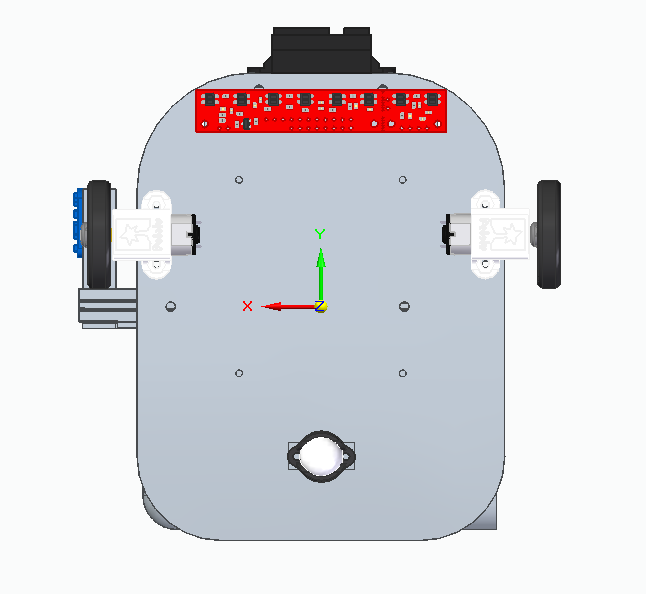
\includegraphics[width=.5\textwidth] {onderkant}
	\caption{Onderaanzicht van het CAD-model}
	\label{fig:Onderkant}
\end{figure}

De Raspberry Pi wordt geplaatst op vier afstandsbussen van 15mm hoog waardoor hij op een platform komt te staan. Dit doen we om wat meer ruimte te creëren voor de sensoren, motoren, wielen en Maker Beams die nog op het chassis moeten komen. Op de Raspberry Pi komen 2  kleine breadboards die aan elkaar gelinkt zijn. Achter de Raspberry Pi ter hoogte van onze Ball Caster zullen we de powerbank op het chassis plaatsen. Deze past jammer genoeg juist niet onder de Raspberry waardoor hij niet onder het platform kan. De powerbank zorgt met zijn gewicht ervoor dat het massamiddelpunt van de wagen meer naar achteren en lager komt te liggen wat zorgt voor extra stabiliteit. De powerbank is ook makkelijk aan te sluiten op de Raspberry Pi en levert het juiste voltage voor de Raspberry Pi om te functioneren. 

\begin{figure}[h]
	\centering
	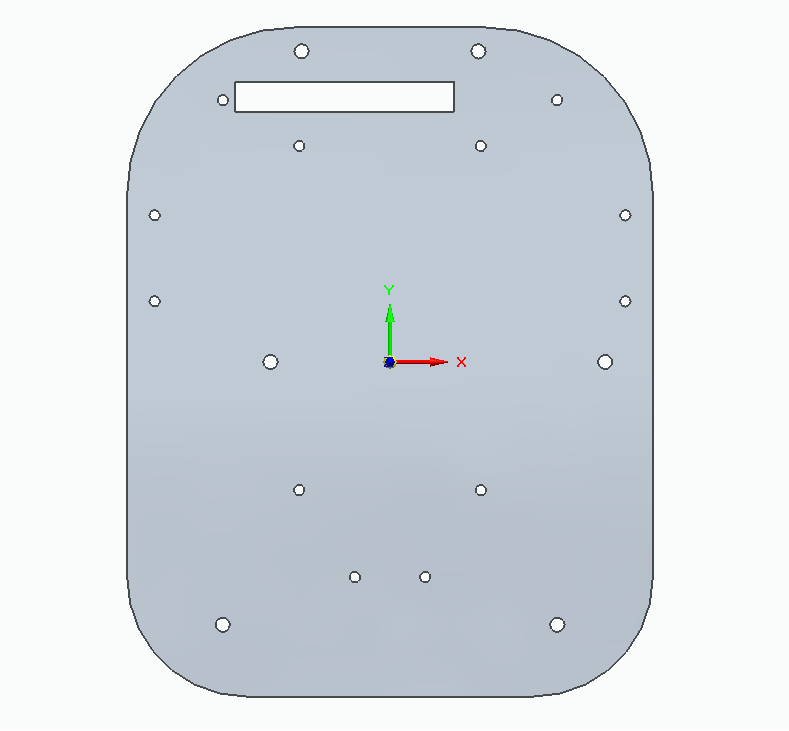
\includegraphics[width=.5\textwidth] {chassis3d}
	\caption{CAD-model van het zelf ontworpen chassis.}
	\label{fig:chassis}
\end{figure}

Het chassis \ref{fig:chassis} is handmatig ontworpen naar de behoeften van het robotwagentje en zal ge-3D-print worden op basis van een doorgestuurd ontwerp door de assistenten van het vak. Dit chassis zal 140 mm lang, 110 mm breed en 3 mm dik zijn met afgeronde hoeken. Hiermee bekomen we een rechthoekig chassis waarmee we genoeg ruimte hebben in de lengte om onze microcontroller en onze powerbank op te plaatsen. De afgeronde hoeken zorgen ervoor dat bochten makkelijker genomen kunnen worden. Vooraan het chassis zal er een gleuf voorzien worden van 6,5 mm breed en 45,8 mm lang voor de verbindingsdraden naar de lijnsensor die onder het chassis hangt. Er zullen ook gaten in het chassis bevinden die kunnen gebruikt worden voor het bevestigen van componenten met schroeven en moeren. Het chassis zal aan een dichtheid van 70\% ge-3D-print worden zodat hij genoeg steun kan bieden en niet zal doorzakken.

\subsection{Sensoren}
De kleurensensor zal bevestigt worden aan een MakerBeam op een hoogte van 75mm van de grond zodat deze het verkeerslicht, die op dezelfde hoogte hangt, kan detecteren. Hierbij zal een constructie van MakerBeams ervoor zorgen dat de kleurensensor kan verplaatst worden in alle richtingen indien nodig. \ref{fig:Linksaanzicht} Deze constructie bestaat uit een MakerBeam die horizontaal in het midden van ons chassis ligt onder de Raspberry Pi met daarop een MakerBeam verticaal omhoog aan het rechter uiteinde. Hierop wordt een  horizontale MakerBeam bevestigt met de kleurensensor eraan.
\begin{figure}[h]
	\centering
	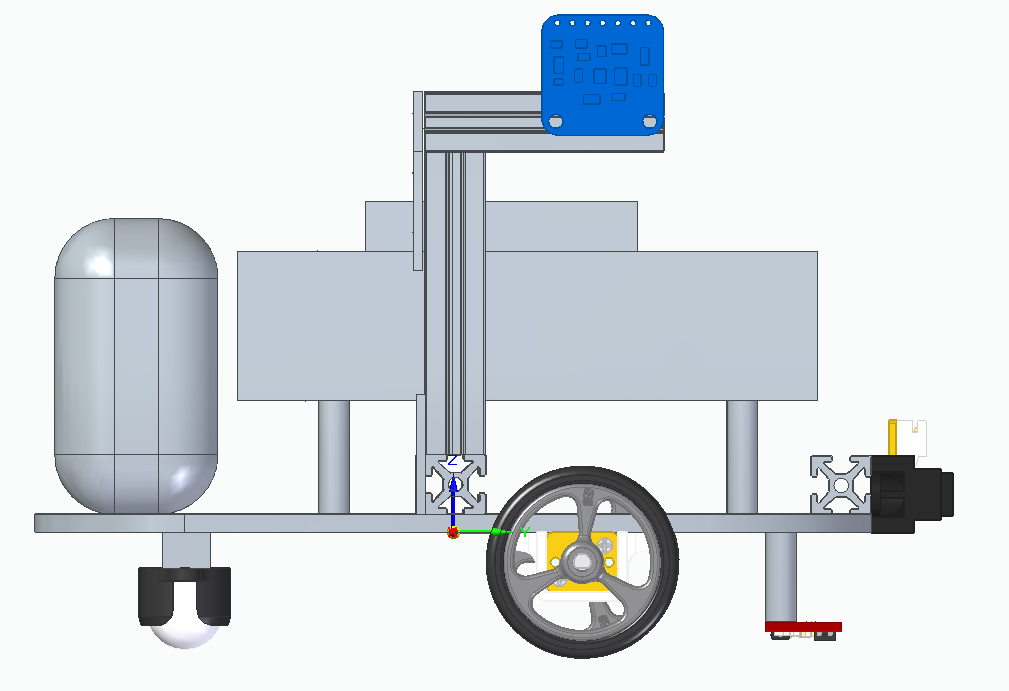
\includegraphics[width=.5\textwidth] {rechterkant}
	\caption{Linkeraanzicht van het CAD-Model met constructie voor kleurensensor op}
	\label{fig:Linksaanzicht}
\end{figure}

Voor de afstandssensor hebben we gekozen voor een analoge sensor, opdat we nauwkeurig kunnen meten hoever het wagentje verwijderd is van een obstakel of een andere weggebruiker. Doordat we dit onderscheid kunnen maken moet onze miniatuur robotwagen niet direct stoppen wanneer hij een voorligger detecteert, maar kan hij er voor  zorgen dat hij eerst wat trager rijdt vooraleer volledig te stoppen. Deze afstandssensor plaatsen we logischer wijze aan de voorkant van ons chassis aan een MakerBeam zodat hij zo vroeg mogelijk een voorligger kan detecteren aangezien zijn detectie bereik maar 100mm is. 

De reflectiesensor wordt gebruikt om de volglijn te detecteren. Hierbij hebben we een digitale sensor gekozen omdat deze compatibel is met de Raspberry Pi microcontroller en de sensor geen onderscheid moet kunnen maken tussen de soort lijn. Deze wordt aan de voorkant onder het chassis bevestigd met behulp van afstandsbuizen zodat deze de volglijn als eerst detecteert en we zo sneller correcties kunnen uitvoeren. Aangezien de sensor dicht bij de wielen ligt zal het wagentje ook nauwkeuriger bewegen.

Het volledige ontwerp is te bewonderen in volgende figuur.\ref{fig:chassis}

\begin{figure}[h]
	\centering
	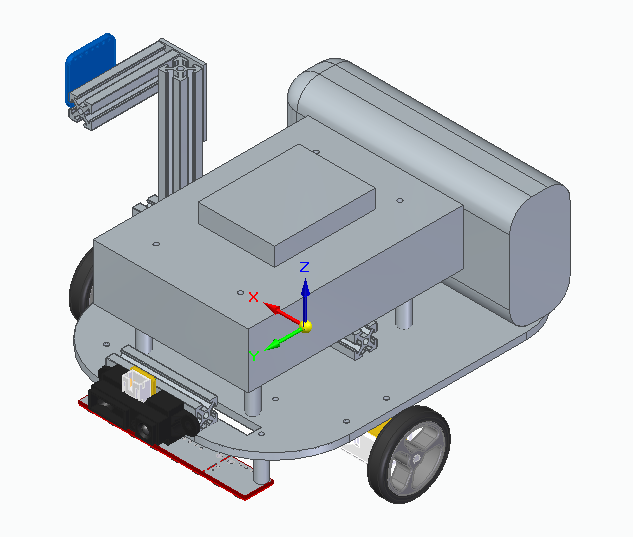
\includegraphics[width=.5\textwidth] {afbchassis}
	\caption{Het volledige CAD-Model}
	\label{fig:chassis}
\end{figure}

\section{Evaluatie}

\subsection{Planning}
Tot en met week 5 is alles verlopen zoals gepland en vastgelegd in de Gantt-grafiek. De documenten met betrekking tot de planning zijn afgewerkt net zoals het ontwerp van de chassis en het CAD-model. Het bestellen van de onderdelen vond later plaats dan verwacht, vanwege de plaatsing bij de bieding. Dit heeft ons met een achterstand doen starten aan het programmeren en assembleren. Het team was van plan om te beginnen met de assemblage in week 6, echter wordt dit een week uitgesteld vanwege een probleem met de microcontroller. Het programmeren van de sensoren verliep vlot, enkel het programmeren in verband met de aansturing van het wagentje zal iets meer tijd innemen dan ingerekend. Dit wordt dan wel gecompenseerd met het maken van het CAD-model dat minder tijd innam dan voorspeld, waardoor we nog altijd op schema zitten. Ook het schrijven van het verslag verloopt volgens schema. De tijd voorzien tijdens de lessen wordt efficiënt gebruikt, waardoor het werk buiten de lessen wordt beperkt tot een minimum.


\subsection{Financiën}

Doordat we de laatste keuze hadden bij het bestellen, liepen we achter op onze planning, onze financiële situatie kende hier dan weer voordelen door. We zijn gestart met een budget van 3500 kredietpunten, dat werd gereduceerd tot een tegoed van 1768 na het plaatsen van een eerste bestelling. In deze  order werden alle grote onderdelen en zaken die we zeker nodig hadden besteld.  Aan onze eerste levering ontbraken nog Maker Beams en afstandsbussen. Onze tweede bestelling zal voorlopig 61 kredietpunten kosten, waardoor we stranden op een budget van 1646 kredietpunten. Door eigen keuze wordt het chassis zelf ontworpen en 3D-geprint. Dit is vermoedelijk een grote kost die werd geschat op 500 kredietpunten. Onze financiële toestand zorgt ervoor dat we in een comfortabele situatie zitten en kunnen we het ons veroorloven om fouten te maken en risico's te nemen. 


\section{Besluit}


Met het gegeven budget hebben we de mogelijkheid een correct functionerend wagentje te bouwen die in staat is autonoom een voorgeprogrammeerd pad te volgen zonder hinder te veroorzaken of de verkeersregels te overtreden. Dit project toont op kleine schaal aan dat een smart city en meer specifiek, zelfrijdende wagens minder utopie en meer werkelijkheid worden.
Zelfrijdende wagens kennen zeker een toekomst en hebben hun nut al meermaals bewezen. De weg naar een wereld met autonome wagens is lang, maar wordt stilaan meer en meer bereden.



	\bibliographystyle{plain} %De stijl van de bibliografie
	\bibliography{bibliografietv} %De bibliografie zelf
\begin{appendices}
	\section*{Planningsdocumenten} %De goede titel
	\renewcommand\refname{} %De oude titel verwijderen
	\vspace{-2\bigskipamount} %De cursor terugzetten
	
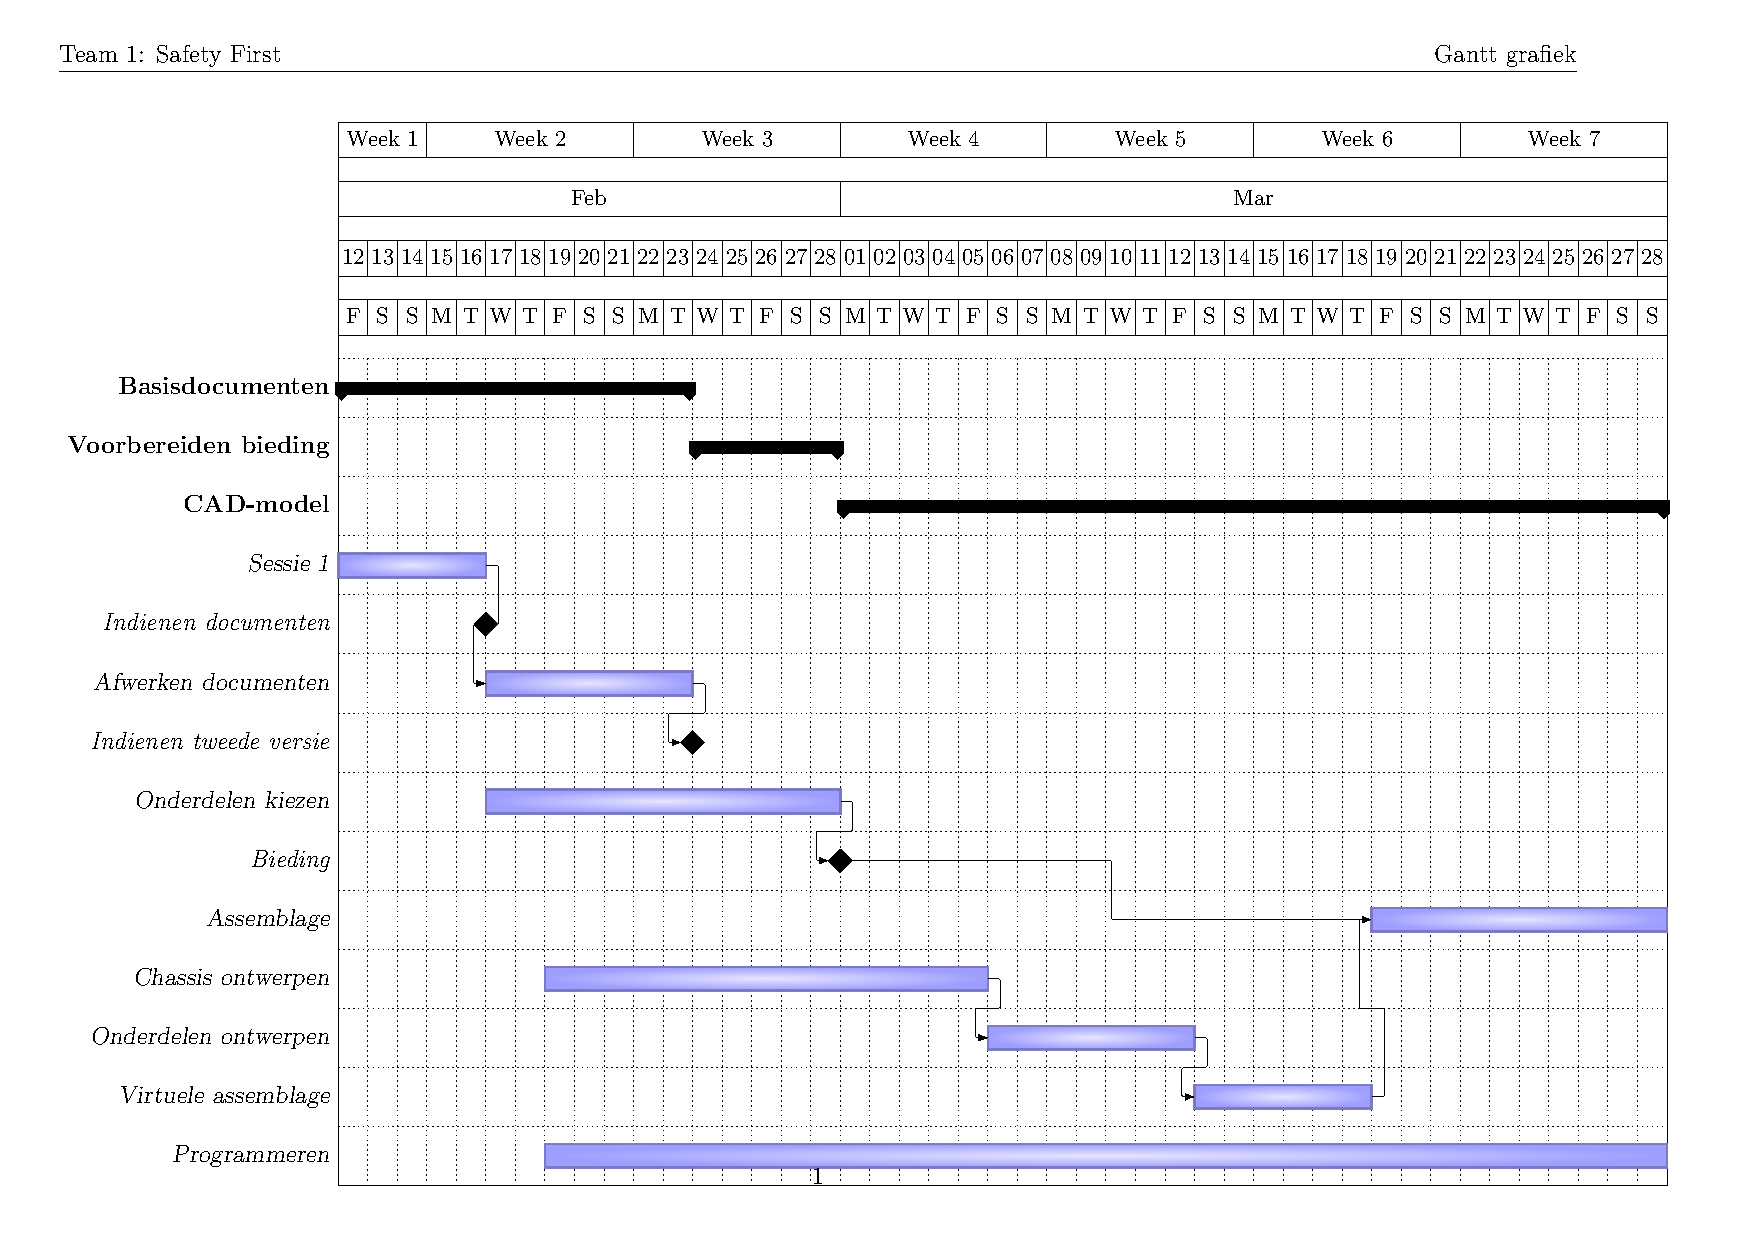
\includepdf[pages=-]{ganttchart.pdf}

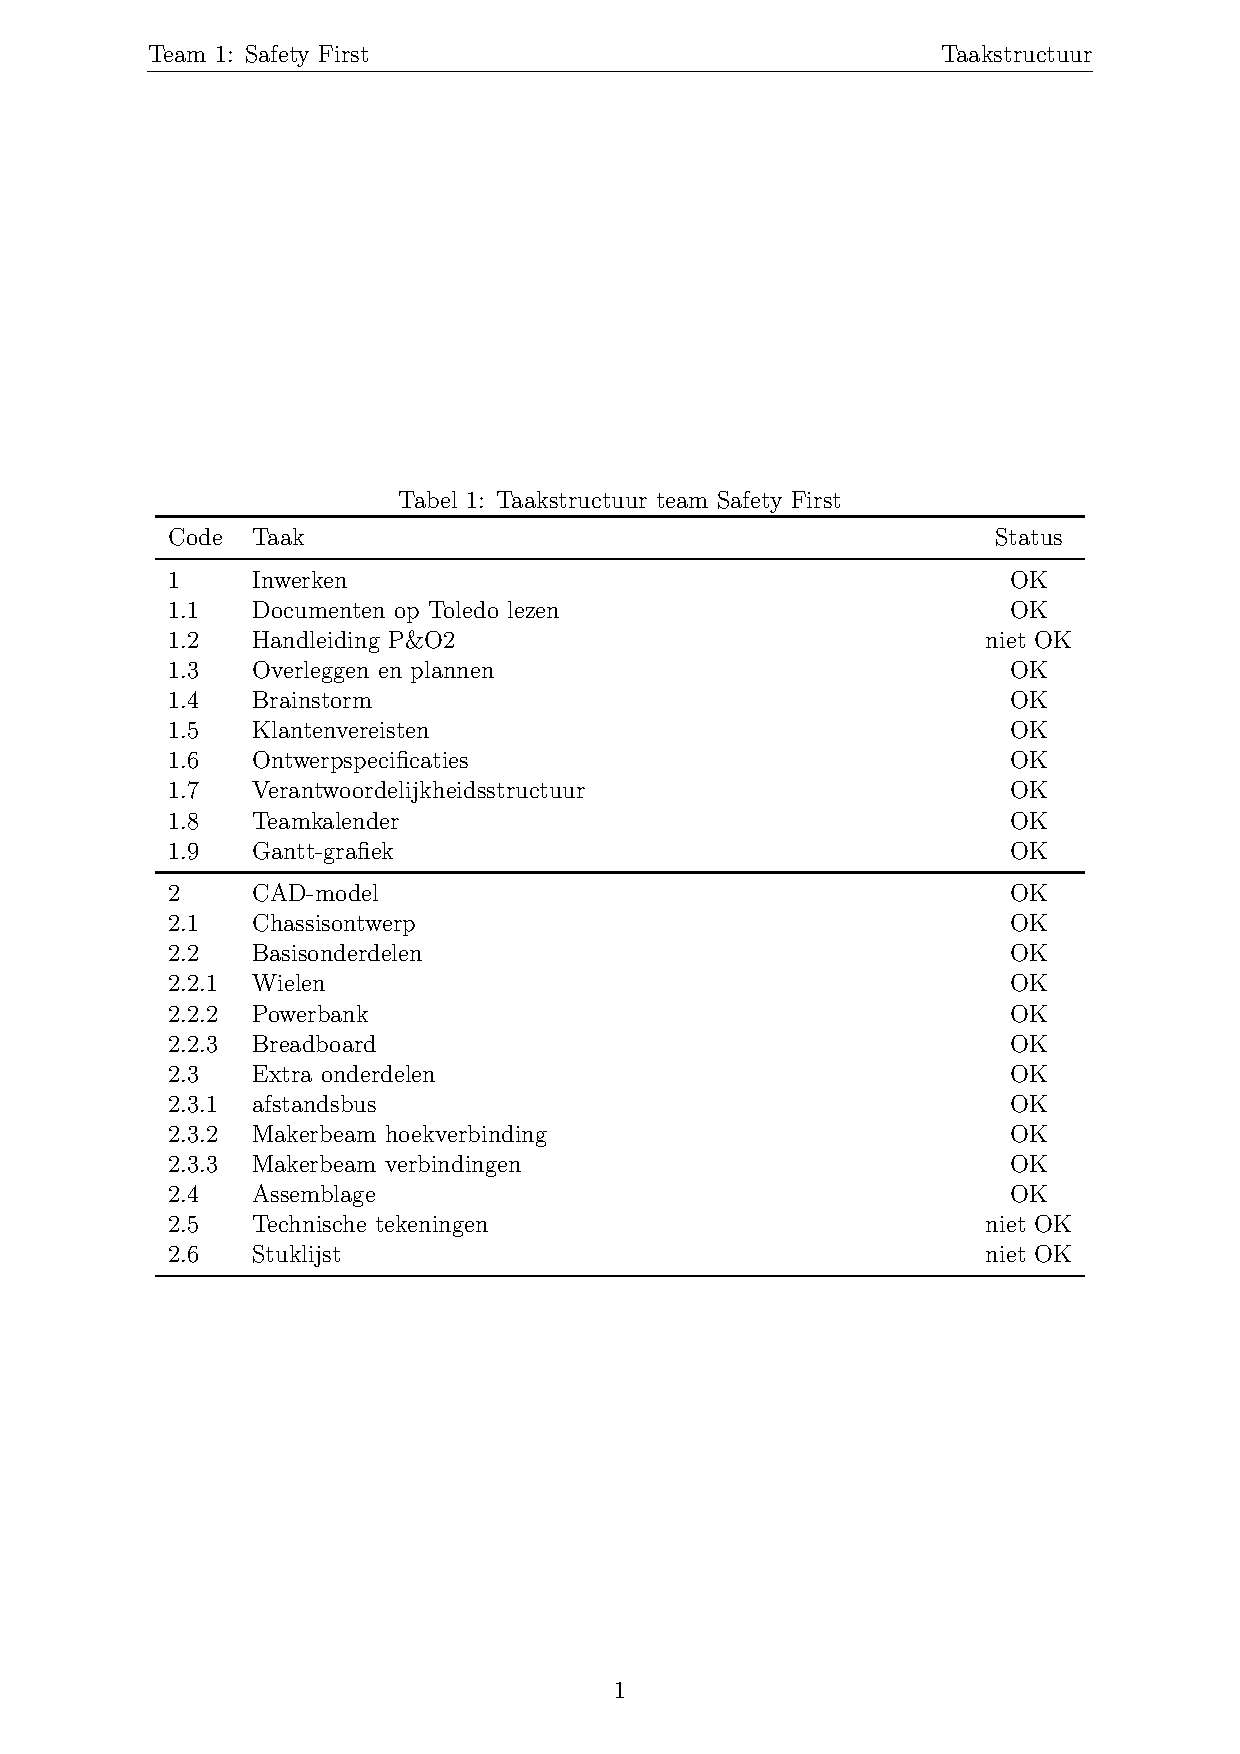
\includepdf[pages=-]{taakstructuur.pdf}

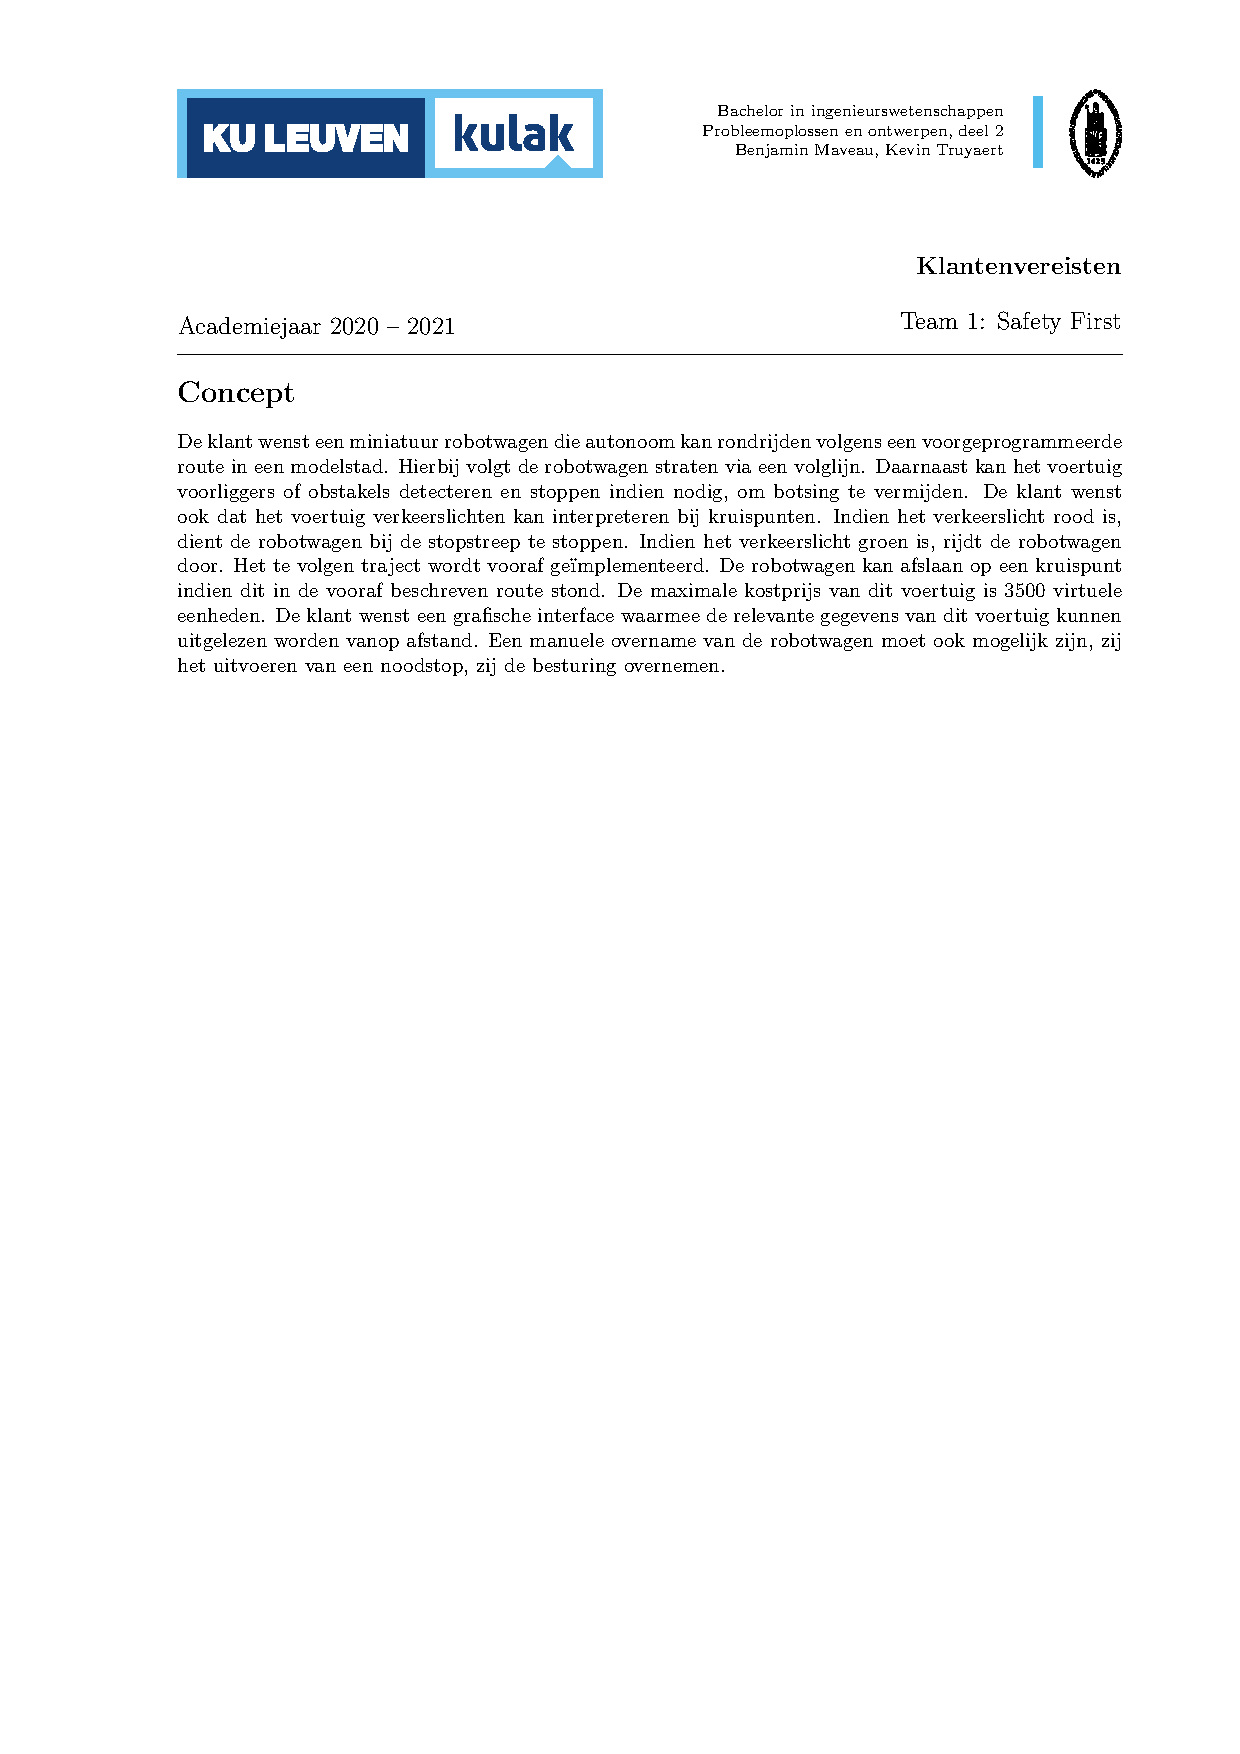
\includepdf[pages=-]{klantenvereisten.pdf}
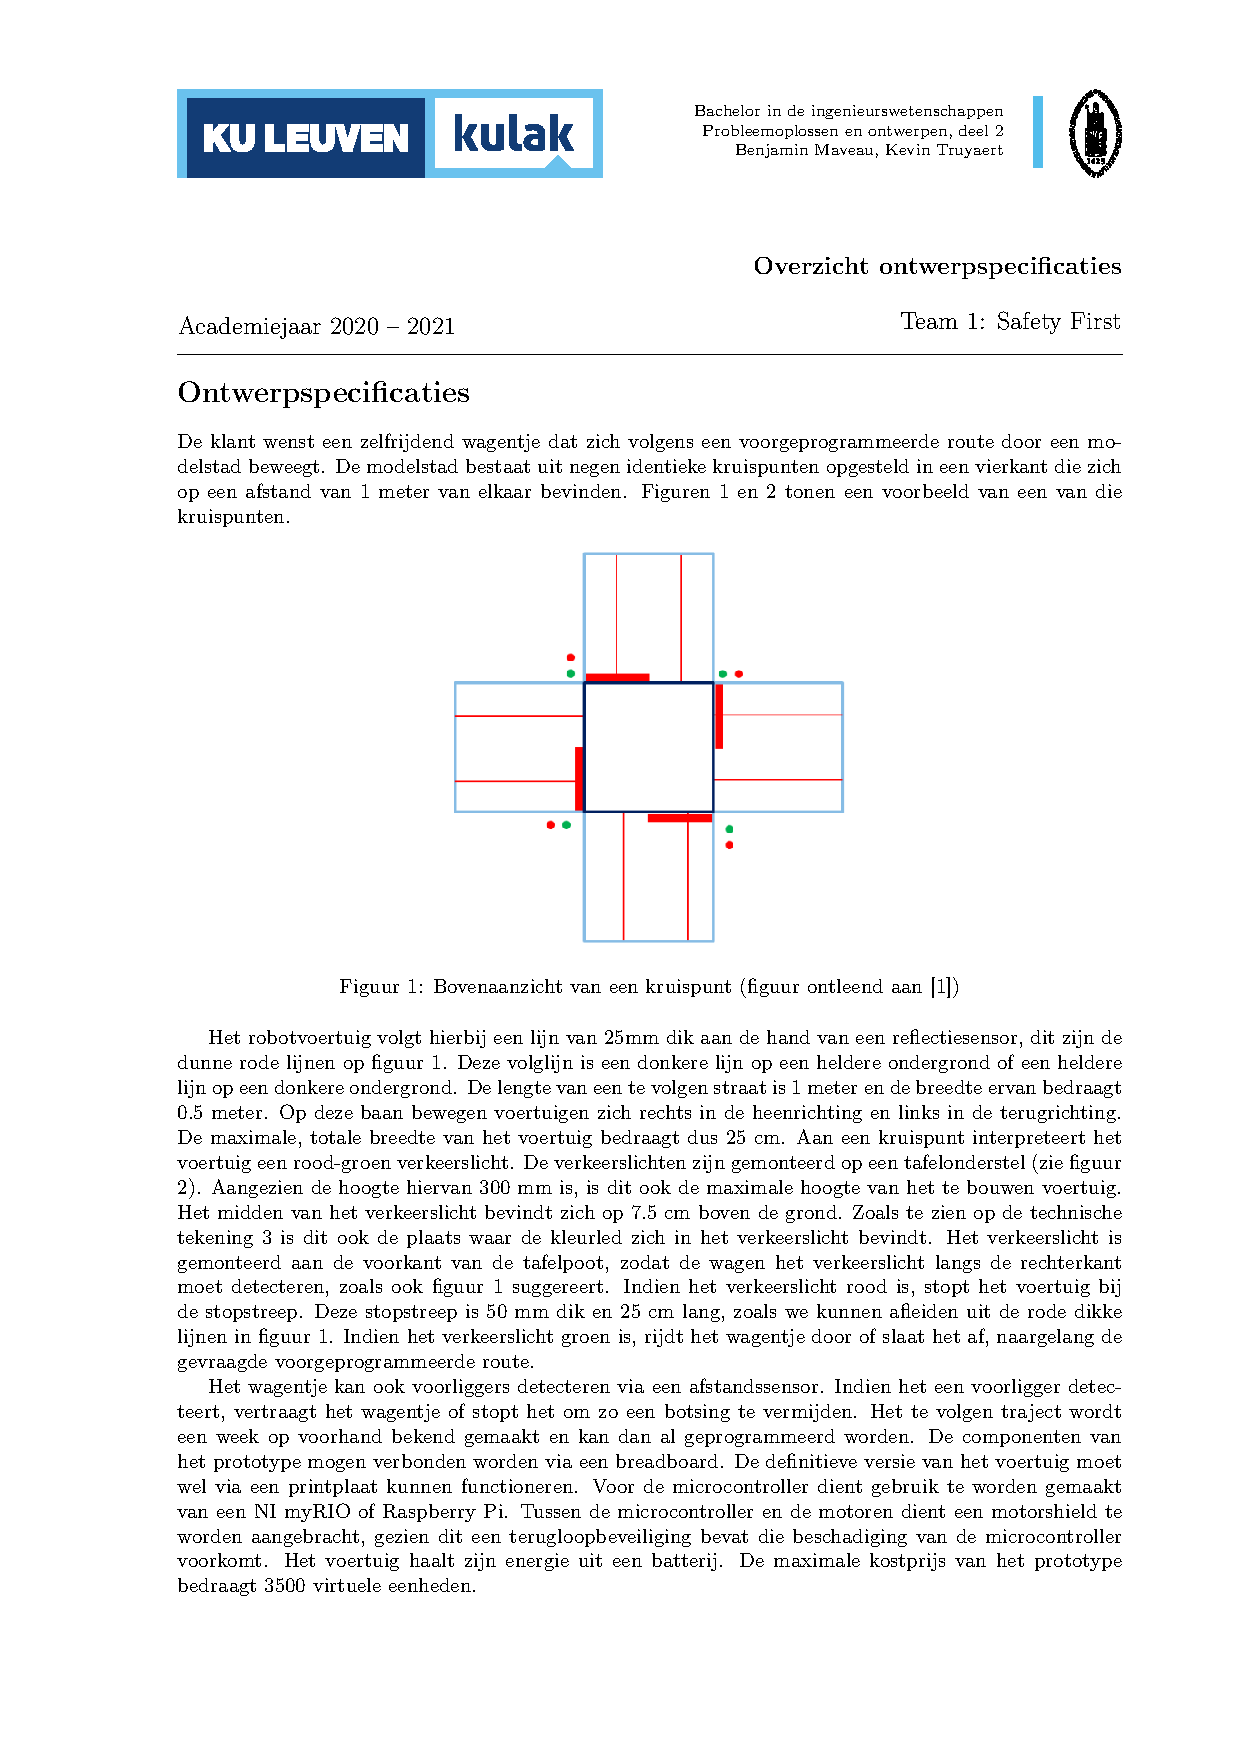
\includepdf[pages=-]{ontwerpspecificaties.pdf}

\end{appendices}




\end{document}